% Created by tikzDevice version 0.6.1 on 2016-06-13 09:09:03
% !TEX encoding = UTF-8 Unicode
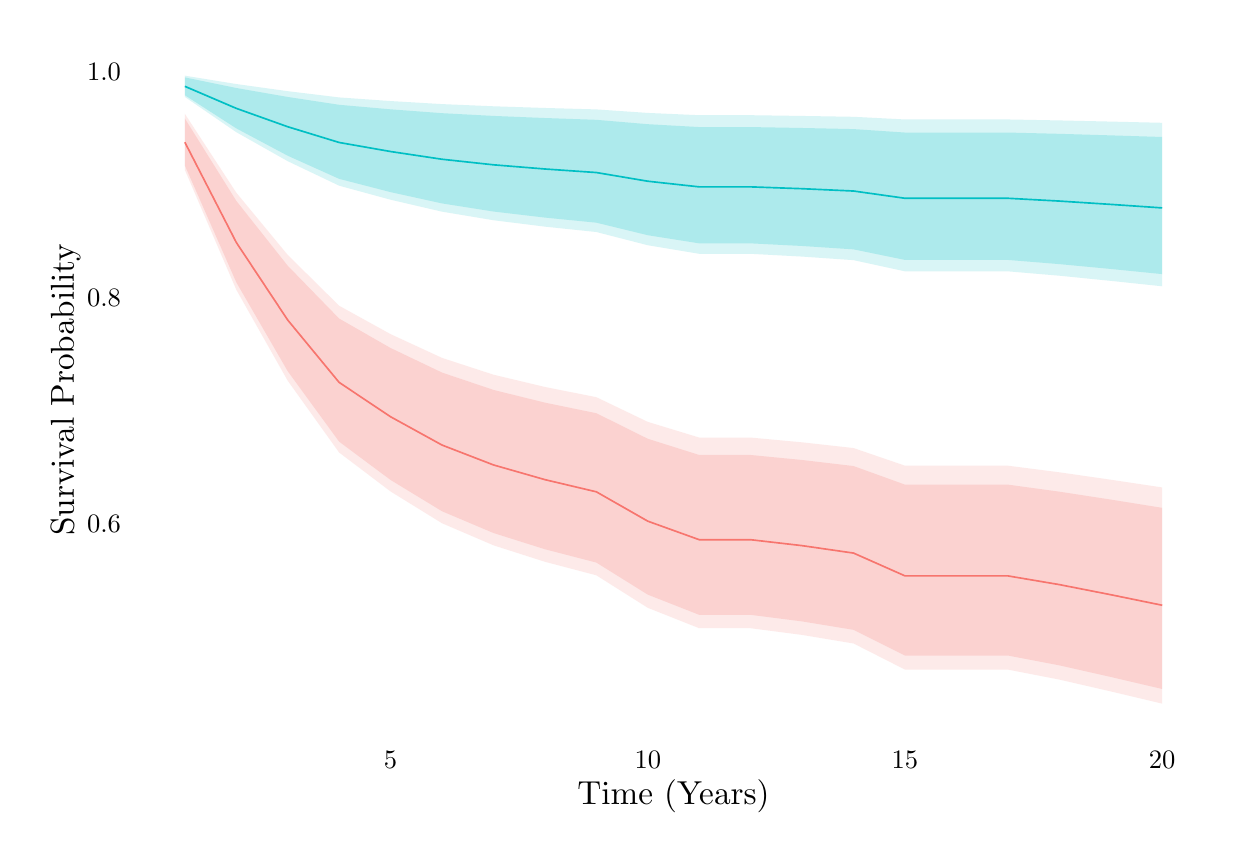
\begin{tikzpicture}[x=1pt,y=1pt]
\definecolor[named]{drawColor}{rgb}{0.00,0.00,0.00}
\definecolor[named]{fillColor}{rgb}{1.00,1.00,1.00}
\fill[color=fillColor,] (0,0) rectangle (433.62,289.08);
\begin{scope}
\path[clip] (  0.00,  0.00) rectangle (433.62,289.08);
\end{scope}
\begin{scope}
\path[clip] (  0.00,  0.00) rectangle (433.62,289.08);
\end{scope}
\begin{scope}
\path[clip] (  0.00,  0.00) rectangle (433.62,289.08);
\end{scope}
\begin{scope}
\path[clip] (  0.00,  0.00) rectangle (433.62,289.08);
\end{scope}
\begin{scope}
\path[clip] (  0.00,  0.00) rectangle (433.62,289.08);
\end{scope}
\begin{scope}
\path[clip] (  0.00,  0.00) rectangle (433.62,289.08);
\end{scope}
\begin{scope}
\path[clip] (  0.00,  0.00) rectangle (433.62,289.08);
\end{scope}
\begin{scope}
\path[clip] (  0.00,  0.00) rectangle (433.62,289.08);
\end{scope}
\begin{scope}
\path[clip] (  0.00,  0.00) rectangle (433.62,289.08);
\end{scope}
\begin{scope}
\path[clip] (  0.00,  0.00) rectangle (433.62,289.08);
\definecolor[named]{drawColor}{rgb}{1.00,1.00,1.00}
\definecolor[named]{fillColor}{rgb}{1.00,1.00,1.00}

\draw[color=drawColor,line width= 0.6pt,line cap=round,line join=round,fill=fillColor,] (  0.00,  0.00) rectangle (433.62,289.08);
\end{scope}
\begin{scope}
\path[clip] (  0.00,  0.00) rectangle (433.62,289.08);
\end{scope}
\begin{scope}
\path[clip] (  0.00,  0.00) rectangle (433.62,289.08);
\end{scope}
\begin{scope}
\path[clip] (  0.00,  0.00) rectangle (433.62,289.08);
\end{scope}
\begin{scope}
\path[clip] ( 39.13, 33.48) rectangle (427.62,283.08);
\definecolor[named]{fillColor}{rgb}{1.00,1.00,1.00}

\draw[fill=fillColor,draw opacity=0.00,] ( 39.13, 33.48) rectangle (427.62,283.08);
\definecolor[named]{drawColor}{rgb}{0.97,0.46,0.43}
\definecolor[named]{fillColor}{rgb}{0.97,0.46,0.43}

\draw[color=drawColor,line width= 0.6pt,line join=round,] ( 56.79,247.68) --
	( 75.38,211.48) --
	( 93.96,183.44) --
	(112.55,160.89) --
	(131.14,148.48) --
	(149.73,138.25) --
	(168.32,131.07) --
	(186.90,125.76) --
	(205.49,121.36) --
	(224.08,110.75) --
	(242.67,104.05) --
	(261.26,104.05) --
	(279.84,101.91) --
	(298.43, 99.22) --
	(317.02, 90.98) --
	(335.61, 90.98) --
	(354.20, 90.98) --
	(372.79, 87.83) --
	(391.37, 84.18) --
	(409.96, 80.37);
\definecolor[named]{drawColor}{rgb}{0.00,0.75,0.77}
\definecolor[named]{fillColor}{rgb}{0.00,0.75,0.77}

\draw[color=drawColor,line width= 0.6pt,line join=round,] ( 56.79,267.88) --
	( 75.38,259.92) --
	( 93.96,253.28) --
	(112.55,247.59) --
	(131.14,244.32) --
	(149.73,241.53) --
	(168.32,239.52) --
	(186.90,238.01) --
	(205.49,236.73) --
	(224.08,233.59) --
	(242.67,231.55) --
	(261.26,231.55) --
	(279.84,230.89) --
	(298.43,230.05) --
	(317.02,227.43) --
	(335.61,227.43) --
	(354.20,227.43) --
	(372.79,226.42) --
	(391.37,225.22) --
	(409.96,223.95);
\definecolor[named]{fillColor}{rgb}{0.97,0.46,0.43}

\draw[fill=fillColor,fill opacity=0.15,draw opacity=0.00,] ( 56.79,257.94) --
	( 75.38,229.45) --
	( 93.96,206.96) --
	(112.55,188.59) --
	(131.14,178.33) --
	(149.73,169.75) --
	(168.32,163.68) --
	(186.90,159.25) --
	(205.49,155.55) --
	(224.08,146.63) --
	(242.67,140.96) --
	(261.26,140.96) --
	(279.84,139.24) --
	(298.43,137.17) --
	(317.02,130.80) --
	(335.61,130.80) --
	(354.20,130.80) --
	(372.79,128.41) --
	(391.37,125.73) --
	(409.96,122.94) --
	(409.96, 44.82) --
	(391.37, 49.24) --
	(372.79, 53.51) --
	(354.20, 57.12) --
	(335.61, 57.12) --
	(317.02, 57.12) --
	(298.43, 66.56) --
	(279.84, 69.65) --
	(261.26, 72.07) --
	(242.67, 72.07) --
	(224.08, 79.44) --
	(205.49, 91.19) --
	(186.90, 96.08) --
	(168.32,102.03) --
	(149.73,110.00) --
	(131.14,121.48) --
	(112.55,135.56) --
	( 93.96,161.53) --
	( 75.38,194.40) --
	( 56.79,237.69) --
	cycle;
\definecolor[named]{fillColor}{rgb}{0.00,0.75,0.77}

\draw[fill=fillColor,fill opacity=0.15,draw opacity=0.00,] ( 56.79,271.73) --
	( 75.38,268.71) --
	( 93.96,266.13) --
	(112.55,263.87) --
	(131.14,262.56) --
	(149.73,261.46) --
	(168.32,260.67) --
	(186.90,260.06) --
	(205.49,259.54) --
	(224.08,258.27) --
	(242.67,257.45) --
	(261.26,257.45) --
	(279.84,257.18) --
	(298.43,256.87) --
	(317.02,255.91) --
	(335.61,255.91) --
	(354.20,255.91) --
	(372.79,255.56) --
	(391.37,255.14) --
	(409.96,254.70) --
	(409.96,195.63) --
	(391.37,197.59) --
	(372.79,199.45) --
	(354.20,201.03) --
	(335.61,201.03) --
	(317.02,201.03) --
	(298.43,205.07) --
	(279.84,206.36) --
	(261.26,207.36) --
	(242.67,207.36) --
	(224.08,210.46) --
	(205.49,215.24) --
	(186.90,217.18) --
	(168.32,219.50) --
	(149.73,222.59) --
	(131.14,226.91) --
	(112.55,231.98) --
	( 93.96,240.84) --
	( 75.38,251.32) --
	( 56.79,264.06) --
	cycle;
\definecolor[named]{fillColor}{rgb}{0.97,0.46,0.43}

\draw[fill=fillColor,fill opacity=0.20,draw opacity=0.00,] ( 56.79,256.27) --
	( 75.38,226.50) --
	( 93.96,203.06) --
	(112.55,183.96) --
	(131.14,173.33) --
	(149.73,164.45) --
	(168.32,158.18) --
	(186.90,153.59) --
	(205.49,149.76) --
	(224.08,140.53) --
	(242.67,134.67) --
	(261.26,134.67) --
	(279.84,132.86) --
	(298.43,130.67) --
	(317.02,123.96) --
	(335.61,123.96) --
	(354.20,123.96) --
	(372.79,121.42) --
	(391.37,118.56) --
	(409.96,115.57) --
	(409.96, 50.11) --
	(391.37, 54.46) --
	(372.79, 58.65) --
	(354.20, 62.20) --
	(335.61, 62.20) --
	(317.02, 62.20) --
	(298.43, 71.48) --
	(279.84, 74.53) --
	(261.26, 76.90) --
	(242.67, 76.90) --
	(224.08, 84.20) --
	(205.49, 95.79) --
	(186.90,100.61) --
	(168.32,106.47) --
	(149.73,114.33) --
	(131.14,125.64) --
	(112.55,139.48) --
	( 93.96,164.95) --
	( 75.38,197.08) --
	( 56.79,239.28) --
	cycle;
\definecolor[named]{fillColor}{rgb}{0.00,0.75,0.77}

\draw[fill=fillColor,fill opacity=0.20,draw opacity=0.00,] ( 56.79,271.11) --
	( 75.38,267.28) --
	( 93.96,264.04) --
	(112.55,261.21) --
	(131.14,259.57) --
	(149.73,258.18) --
	(168.32,257.19) --
	(186.90,256.43) --
	(205.49,255.78) --
	(224.08,254.20) --
	(242.67,253.16) --
	(261.26,253.16) --
	(279.84,252.83) --
	(298.43,252.43) --
	(317.02,251.18) --
	(335.61,251.18) --
	(354.20,251.18) --
	(372.79,250.72) --
	(391.37,250.16) --
	(409.96,249.58) --
	(409.96,200.03) --
	(391.37,201.89) --
	(372.79,203.64) --
	(354.20,205.15) --
	(335.61,205.15) --
	(317.02,205.15) --
	(298.43,208.97) --
	(279.84,210.19) --
	(261.26,211.14) --
	(242.67,211.14) --
	(224.08,214.08) --
	(205.49,218.61) --
	(186.90,220.45) --
	(168.32,222.64) --
	(149.73,225.57) --
	(131.14,229.65) --
	(112.55,234.45) --
	( 93.96,242.81) --
	( 75.38,252.69) --
	( 56.79,264.67) --
	cycle;
\end{scope}
\begin{scope}
\path[clip] (  0.00,  0.00) rectangle (433.62,289.08);
\end{scope}
\begin{scope}
\path[clip] (  0.00,  0.00) rectangle (433.62,289.08);
\end{scope}
\begin{scope}
\path[clip] (  0.00,  0.00) rectangle (433.62,289.08);
\end{scope}
\begin{scope}
\path[clip] (  0.00,  0.00) rectangle (433.62,289.08);
\end{scope}
\begin{scope}
\path[clip] (  0.00,  0.00) rectangle (433.62,289.08);
\end{scope}
\begin{scope}
\path[clip] (  0.00,  0.00) rectangle (433.62,289.08);
\definecolor[named]{drawColor}{rgb}{0.00,0.00,0.00}

\node[color=drawColor,anchor=base east,inner sep=0pt, outer sep=0pt, scale=  0.96] at ( 33.73,106.51) {0.6%
};

\node[color=drawColor,anchor=base east,inner sep=0pt, outer sep=0pt, scale=  0.96] at ( 33.73,188.16) {0.8%
};

\node[color=drawColor,anchor=base east,inner sep=0pt, outer sep=0pt, scale=  0.96] at ( 33.73,269.81) {1.0%
};
\end{scope}
\begin{scope}
\path[clip] (  0.00,  0.00) rectangle (433.62,289.08);
\end{scope}
\begin{scope}
\path[clip] (  0.00,  0.00) rectangle (433.62,289.08);
\end{scope}
\begin{scope}
\path[clip] (  0.00,  0.00) rectangle (433.62,289.08);
\end{scope}
\begin{scope}
\path[clip] (  0.00,  0.00) rectangle (433.62,289.08);
\end{scope}
\begin{scope}
\path[clip] (  0.00,  0.00) rectangle (433.62,289.08);
\end{scope}
\begin{scope}
\path[clip] (  0.00,  0.00) rectangle (433.62,289.08);
\end{scope}
\begin{scope}
\path[clip] (  0.00,  0.00) rectangle (433.62,289.08);
\end{scope}
\begin{scope}
\path[clip] (  0.00,  0.00) rectangle (433.62,289.08);
\end{scope}
\begin{scope}
\path[clip] (  0.00,  0.00) rectangle (433.62,289.08);
\end{scope}
\begin{scope}
\path[clip] (  0.00,  0.00) rectangle (433.62,289.08);
\end{scope}
\begin{scope}
\path[clip] (  0.00,  0.00) rectangle (433.62,289.08);
\end{scope}
\begin{scope}
\path[clip] (  0.00,  0.00) rectangle (433.62,289.08);
\definecolor[named]{drawColor}{rgb}{0.00,0.00,0.00}

\node[color=drawColor,anchor=base,inner sep=0pt, outer sep=0pt, scale=  0.96] at (131.14, 21.46) {5%
};

\node[color=drawColor,anchor=base,inner sep=0pt, outer sep=0pt, scale=  0.96] at (224.08, 21.46) {10%
};

\node[color=drawColor,anchor=base,inner sep=0pt, outer sep=0pt, scale=  0.96] at (317.02, 21.46) {15%
};

\node[color=drawColor,anchor=base,inner sep=0pt, outer sep=0pt, scale=  0.96] at (409.96, 21.46) {20%
};
\end{scope}
\begin{scope}
\path[clip] (  0.00,  0.00) rectangle (433.62,289.08);
\end{scope}
\begin{scope}
\path[clip] (  0.00,  0.00) rectangle (433.62,289.08);
\end{scope}
\begin{scope}
\path[clip] (  0.00,  0.00) rectangle (433.62,289.08);
\end{scope}
\begin{scope}
\path[clip] (  0.00,  0.00) rectangle (433.62,289.08);
\definecolor[named]{drawColor}{rgb}{0.00,0.00,0.00}

\node[color=drawColor,anchor=base,inner sep=0pt, outer sep=0pt, scale=  1.20] at (233.37,  8.40) {Time (Years)%
};
\end{scope}
\begin{scope}
\path[clip] (  0.00,  0.00) rectangle (433.62,289.08);
\end{scope}
\begin{scope}
\path[clip] (  0.00,  0.00) rectangle (433.62,289.08);
\definecolor[named]{drawColor}{rgb}{0.00,0.00,0.00}

\node[rotate= 90.00,color=drawColor,anchor=base,inner sep=0pt, outer sep=0pt, scale=  1.20] at ( 16.66,158.28) {Survival Probability%
};
\end{scope}
\begin{scope}
\path[clip] (  0.00,  0.00) rectangle (433.62,289.08);
\end{scope}
\begin{scope}
\path[clip] (  0.00,  0.00) rectangle (433.62,289.08);
\end{scope}
\begin{scope}
\path[clip] (  0.00,  0.00) rectangle (433.62,289.08);
\end{scope}
\begin{scope}
\path[clip] (  0.00,  0.00) rectangle (433.62,289.08);
\end{scope}
\end{tikzpicture}
